\subsection{Постановка задачи}
4.2. Реализовать метод стрельбы и конечно-разностный метод решения краевой задачи для ОДУ в виде программ. С использованием разработанного программного обеспечения решить краевую задачу для обыкновенного дифференциального уравнения 2-го порядка на указанном отрезке. Оценить погрешность численного решения с использованием метода Рунге – Ромберга и путем сравнения с точным решением. 

{\bfseries Вариант:} 19
    \begin{equation}
		y'' + 4xy' +(4x^2 + 2)y = 0,\\
		y'(0)=1,\\
		4y(2)-y'(2)=23e^{-4}
    \end{equation}
    
    \begin{equation}
		y(x) = (1+x)e^{-x^2}
    \end{equation}
\pagebreak

\subsection{Результаты работы}
\begin{figure}[h!]
\centering
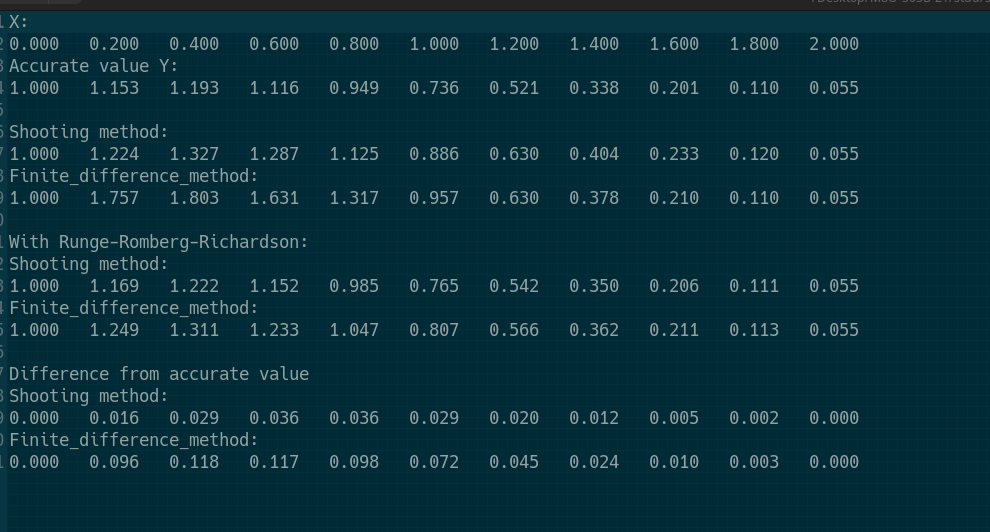
\includegraphics[width=.7\textwidth]{lab4.2}
\caption{Вывод в консоли}
\end{figure}


\subsection{Исходный код}
\lstinputlisting[title=\texttt{Lab4.2.cpp}]{../stud/saifullin/task4.2/Lab4.2.cpp}
\pagebreak

